\section{ λ-Calculus? }

\frame{\frametitle{Table of Contents}
  \begin{itemize}
    \item {\color{lightgray}What can Haskell do?}
    \item {What is λ-Calculus?}
    \item {\color{lightgray} Why Implement λ-Calculus?}
    \item {\color{lightgray} Let's Implement λ-Calculus}
    \item {\color{lightgray} Questions?}
    \item {\color{lightgray} References}
  \end{itemize}
}

%\ftc{λ-Calculus?}
\frame{\frametitle{λ-Calculus?}
\begin{itemize}
  \item[] {}
  \item[] {}
  \item[] {An important formal system}
  \item[] {for functional programming}
  \item[] {}
  \item[] {}
\end{itemize}
}

\subsection{Turing Machine}
% \ftc{Turing Machine}

\frame{\frametitle{Turing Machine}
  \begin{itemize}
  \item[]{}
  \item[]{}
  \item{[Turing machine picture]}
  \item{Invented by Alan Turing in 1936}
  \item[]{}
  \item[]{}
  \end{itemize}
}

\frame{\frametitle{Turing Machine}
  \begin{itemize}
    \item<1->{\normalsize Infinite {\color{darkblue}tape} which stores symbols {\small(memory)}}
    \item<2->{\normalsize Finite {\color{darkblue}action table} which represents\\{\small (state, symbol) $\to$ action (program)}}
    \item<3->{\normalsize {\color{darkblue}Robotic arm} {\small (CPU with a register which stores current state)}
      \begin{itemize}
      \item<4->{\small Read the symbol on the tape at current position}
      \item<5->{\small Write a symbol on the tape at current position}
      \item<6->{\small Move the tape left or right}
      \end{itemize}
    }
  \end{itemize}
}

\frame{\frametitle{Turing Complete}
  \begin{itemize}
    \item[]{}
    \item[]{}
    \item<1->{Whatever Turing machine can do}
    \item<2>{So what is λ-calculus?}
    \item[]{}
    \item[]{}
  \end{itemize}
}

\frame{\frametitle{Alligator Eggs!}
  \begin{figure}[h!]
    \centering
      
\includegraphics[width=0.85\textwidth]{image/eating.png}
      \caption{\jref{http://worrydream.com/AlligatorEggs/}{http://worrydream.com/AlligatorEggs/}}
  \end{figure}
}

\subsection{λ-Calculus}

\frame{\frametitle{λ-Calculus}
\begin{itemize}
  \item[]{}
  \item[]{}
  \item<1->{Invented by Alonzo Church in 1930s}
  \item<2>{Also Turing complete, but how do we prove that?}
  \item[]{}
  \item[]{}
\end{itemize}
}

\frame{\frametitle{λ-Complete}
\begin{itemize}
  \item<1->{\normalsize Whatever λ-calculus can do}
  \item<2->{\normalsize Implement Turing machine in λ-calculus
    \begin{figure}[h!]
      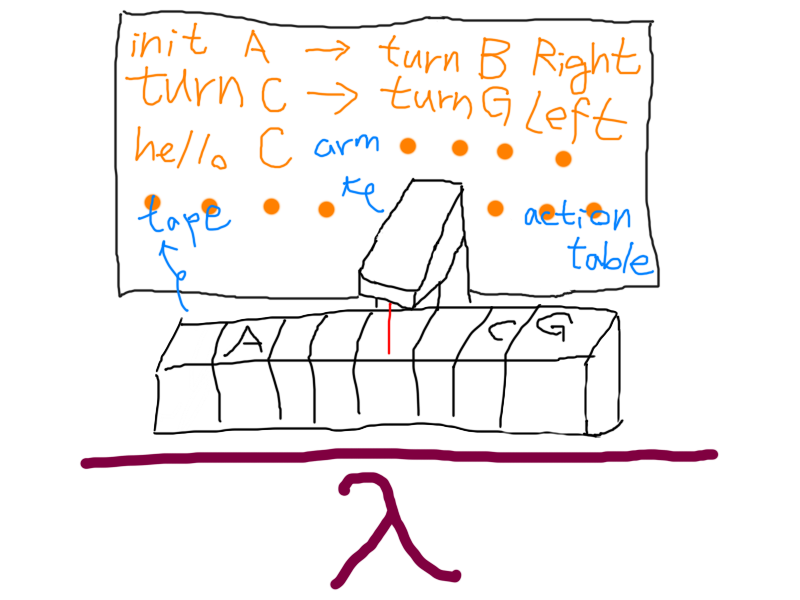
\includegraphics[width=0.55\textwidth]{image/turing-machine-lambda.png}
      % \caption{Turing machine on λ-calculus picture}
    \end{figure}
  }
\end{itemize}
}
\frame{\frametitle{λ-Complete}
\begin{itemize}
  \item<1->{\normalsize So λ-calculus can do anything Turing machine can do}
  \item<2->{\normalsize Plus what λ-calculus can do without a Turing machine}
  \item<3->{\normalsize Thus λ-calculus is Turing complete}
\end{itemize}
}
\frame{\frametitle{λ-Complete}
\begin{itemize}
  \item<1->{\normalsize Implement λ-calculus in Turing machine
    \begin{figure}[h!]
      
\includegraphics[width=0.4\textwidth]{image/eating.png}
      % \caption{λ-calculus on Turing machine picture}
    \end{figure}
  }
  \item<2->{\normalsize So Turing machine is also λ-complete}
\end{itemize}
}
\frame{\frametitle{λ-Complete}
\begin{itemize}
  \item<1->{\normalsize They have the same computability
    \begin{figure}[h!]
      
\includegraphics[width=0.4\textwidth]{image/eating.png}
      % \caption{Turing machine on λ-calculus on Turing machine on ... on λ-calculus on picture}
    \end{figure}
  }\item[] {}
\end{itemize}
}

\frame{\frametitle{What exactly is λ-calculus?}
\begin{itemize}
  \item[]{}
  \item<1->{\usebeamerfont*{font DejaVu Sans Mono} (λx. x+1)}
  \item<2->{\usebeamerfont*{font DejaVu Sans Mono} (λx. x+1) 1}
  \item<3->{\usebeamerfont*{font DejaVu Sans Mono} = (1+1)}
  \item<4->{\usebeamerfont*{font DejaVu Sans Mono} = 2}
  \item[]{}
  \item[]{}
\end{itemize}
}

\frame{\frametitle{Does it look like Lisp?}
\begin{itemize}
  \item[]{}
  \item[]{}
  \item<1->{\usebeamerfont*{font DejaVu Sans Mono} (λf.(λx.f (x x)) (λx.f (x x)))}
  \item[]{}
  \item[]{}
  \item[]{}
\end{itemize}
}

\subsection{Church Encoding}
\ftc{Church Encoding}

\frame{\frametitle{Natural Numbers}
\begin{itemize}
  \item{\usebeamerfont*{font DejaVu Sans Mono} 0 ≡ λf.λx. x}
  \item{\usebeamerfont*{font DejaVu Sans Mono} 1 ≡ λf.λx. f x}
  \item{\usebeamerfont*{font DejaVu Sans Mono} ...}
  \item{\usebeamerfont*{font DejaVu Sans Mono} n ≡ λf.λx. f$^{\text{n}}$ x}
\end{itemize}
}

\frame{\frametitle{Computation with Natural Numbers}
\begin{itemize}
  \item{\usebeamerfont*{font DejaVu Sans Mono} succ ≡ λn.λf.λx. f (n f x)}
  \item{\usebeamerfont*{font DejaVu Sans Mono} plus ≡ λm.λn.λf.λx. m f (n f x)}
\end{itemize}
}

\frame{\frametitle{Booleans}
\begin{itemize}
  \item{\usebeamerfont*{font DejaVu Sans Mono} true \ ≡ λa.λb. a}
  \item{\usebeamerfont*{font DejaVu Sans Mono} false ≡ λa.λb. b}
\end{itemize}
}

\frame{\frametitle{Computation with Booleans}
\begin{itemize}
  \item{\usebeamerfont*{font DejaVu Sans Mono} and ≡ λm.λn. m n m}
  \item{\usebeamerfont*{font DejaVu Sans Mono} or \ ≡ λm.λn. m m n}
  \item{\usebeamerfont*{font DejaVu Sans Mono} not ≡ λm.λa.λb. m b a}
  \item{\usebeamerfont*{font DejaVu Sans Mono} if \ ≡ λm.λa.λb. m a b}
\end{itemize}
}

\subsection{}

\frame{
\vskip 10mm%
\frametitlecenter{Recursion?\\
\usebeamerfont*{font DejaVu Sans Mono}
%{\usebeamerfont*{font Hiragino Maru Gothic}の} %No
No problems!}
}

\subsection{Y combinator}

\frame{\frametitle{Y combinator}
\begin{itemize}
  \item{Discovered by Haskell Curry}
  \item{\normalsize\usebeamerfont*{font DejaVu Sans Mono} y \ \ = λf.(λx.f (x x)) (λx.f (x x))}
  \item{\normalsize\usebeamerfont*{font DejaVu Sans Mono} y f = (λf.(λx.f (x x)) (λx.f (x x))) f}
  \item{\normalsize\usebeamerfont*{font DejaVu Sans Mono} y f = f (y f)}
\end{itemize}
}

\frame{
\vskip 22mm%
\frametitlecenter{{\color{black} Paul Graham},\\I know what is\\Y combinator!}
}

\subsection{Fixed Point Combinator}

\frame{\frametitle{Fixed Point Combinator}
\begin{itemize}
  \item{\normalsize Strict languages need some delay}
  \item{\footnotesize\usebeamerfont*{font DejaVu Sans Mono} Z = (λx.f (λv.((x x) v))) (λx.f (λv.((x x) v)))}
  \item{\normalsize Discovered by Alan Turing}
  \item{\footnotesize\usebeamerfont*{font DejaVu Sans Mono} Θ = (λx.λy. (y (x x y))) (λx.λy. (y (x x y)))}
  \item{\normalsize Constructed by Jan Willem Klop}
  \item{\footnotesize\usebeamerfont*{font DejaVu Sans Mono} Yk = (L L L L L L L L L L L . . .)
    \begin{itemize}
      \item{\tiny\usebeamerfont*{font DejaVu Sans Mono} L = λabcdefghijklmnopqstuvwxyzr. (r (thisisafixedpointcombinator))}
    \end{itemize}
  }
\end{itemize}
}
